\subsection{Baseline predictions}

We began by establishing a baseline model for bass guitar tablature generation.
Initially, we used a pre-trained checkpoint from the DadaGP paper~\cite{sarmento_dadagp_2021} without additional training.
To generate bass-specific outputs, we experimented with prompts containing single or several bass guitar tokens.
Regardless of the number of bass notes given as initial prompt tokens, the model quickly incorporated tokens from other instruments.
This is an issue documented in GTR-CTRL~\cite{sarmento_gtr-ctrl_2023} where they used a metric called the UIP score (Unpromped Instrument Presence) to evaluate the model's ability to generate a specific combinations of instruments.
To constrain the output to bass tokens, we modified the logits of non-bass instruments by setting them to $-\infty$.

% FIGURE REPETITIVE GENERATION
\begin{figure}[!ht]
    \centering
    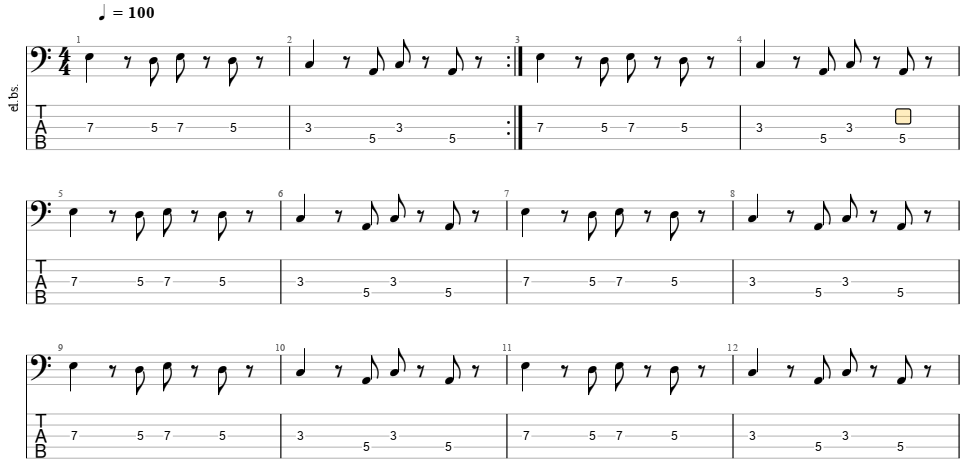
\includegraphics[width=.8\linewidth]{../images-figures/generated_bass_baseline.png}
    \caption{Example of a bass generation from the baseline model}
    \label{fig:repetitive_generation}
\end{figure}

An example of a bass tablature generated this way is shown in Figure~\ref{fig:repetitive_generation}.
The generated part repeats the same patterns of two measures over the entire sequence.
This part could be used as a simple accompaniment but this model lacks the ability to adapt to the tonality of the song and its rhythm.
While this forced the model to generate only bass tokens, the output quality was poor, featuring repetitive phrases, harmonically incorrect notes, or complete aberrations.
This was expected, as the model was not trained explicitly for bass only generation. 

% \newpage

\subsection{BiLSTM - Transformer model}

This section present the results we get using a model adapted from the work of Makris et al.~\cite{makris_conditional_2022}.
Our data was adapted to fit the model's input requirements and the model was also slightly modified to fit our task.

% FIGURE MAKRIS ET AL. MODEL
\begin{figure}[!ht]
    \centering
    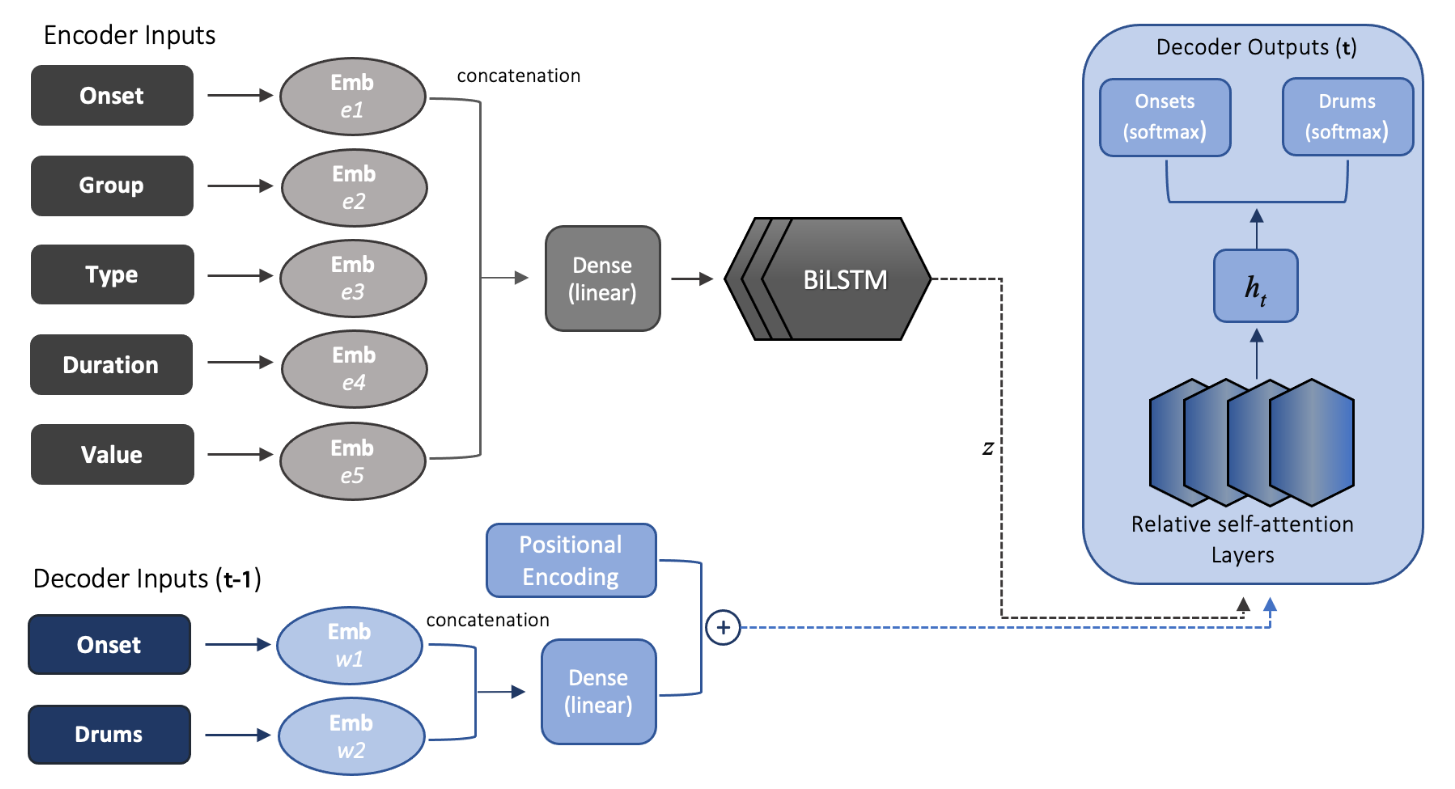
\includegraphics[width=.75\linewidth]{../images-figures/makris_model.png}
    \caption{Makris et al. model architecture, taken from their paper~\cite{makris_conditional_2022}}
    \label{fig:makris_model}
\end{figure}

Figure~\ref{fig:makris_model} shows the architecture of the model proposed by Makris et al.
We have presented the compound representation in the state of the art.
This representation concatenates all the parameters necessary to describe a note in a single vector (onset, duration, pitch etc.).

% FIGURE MAKRIS ET AL. MODEL ADAPTED TO OUR TASK
\begin{figure}[!ht]
    \centering
    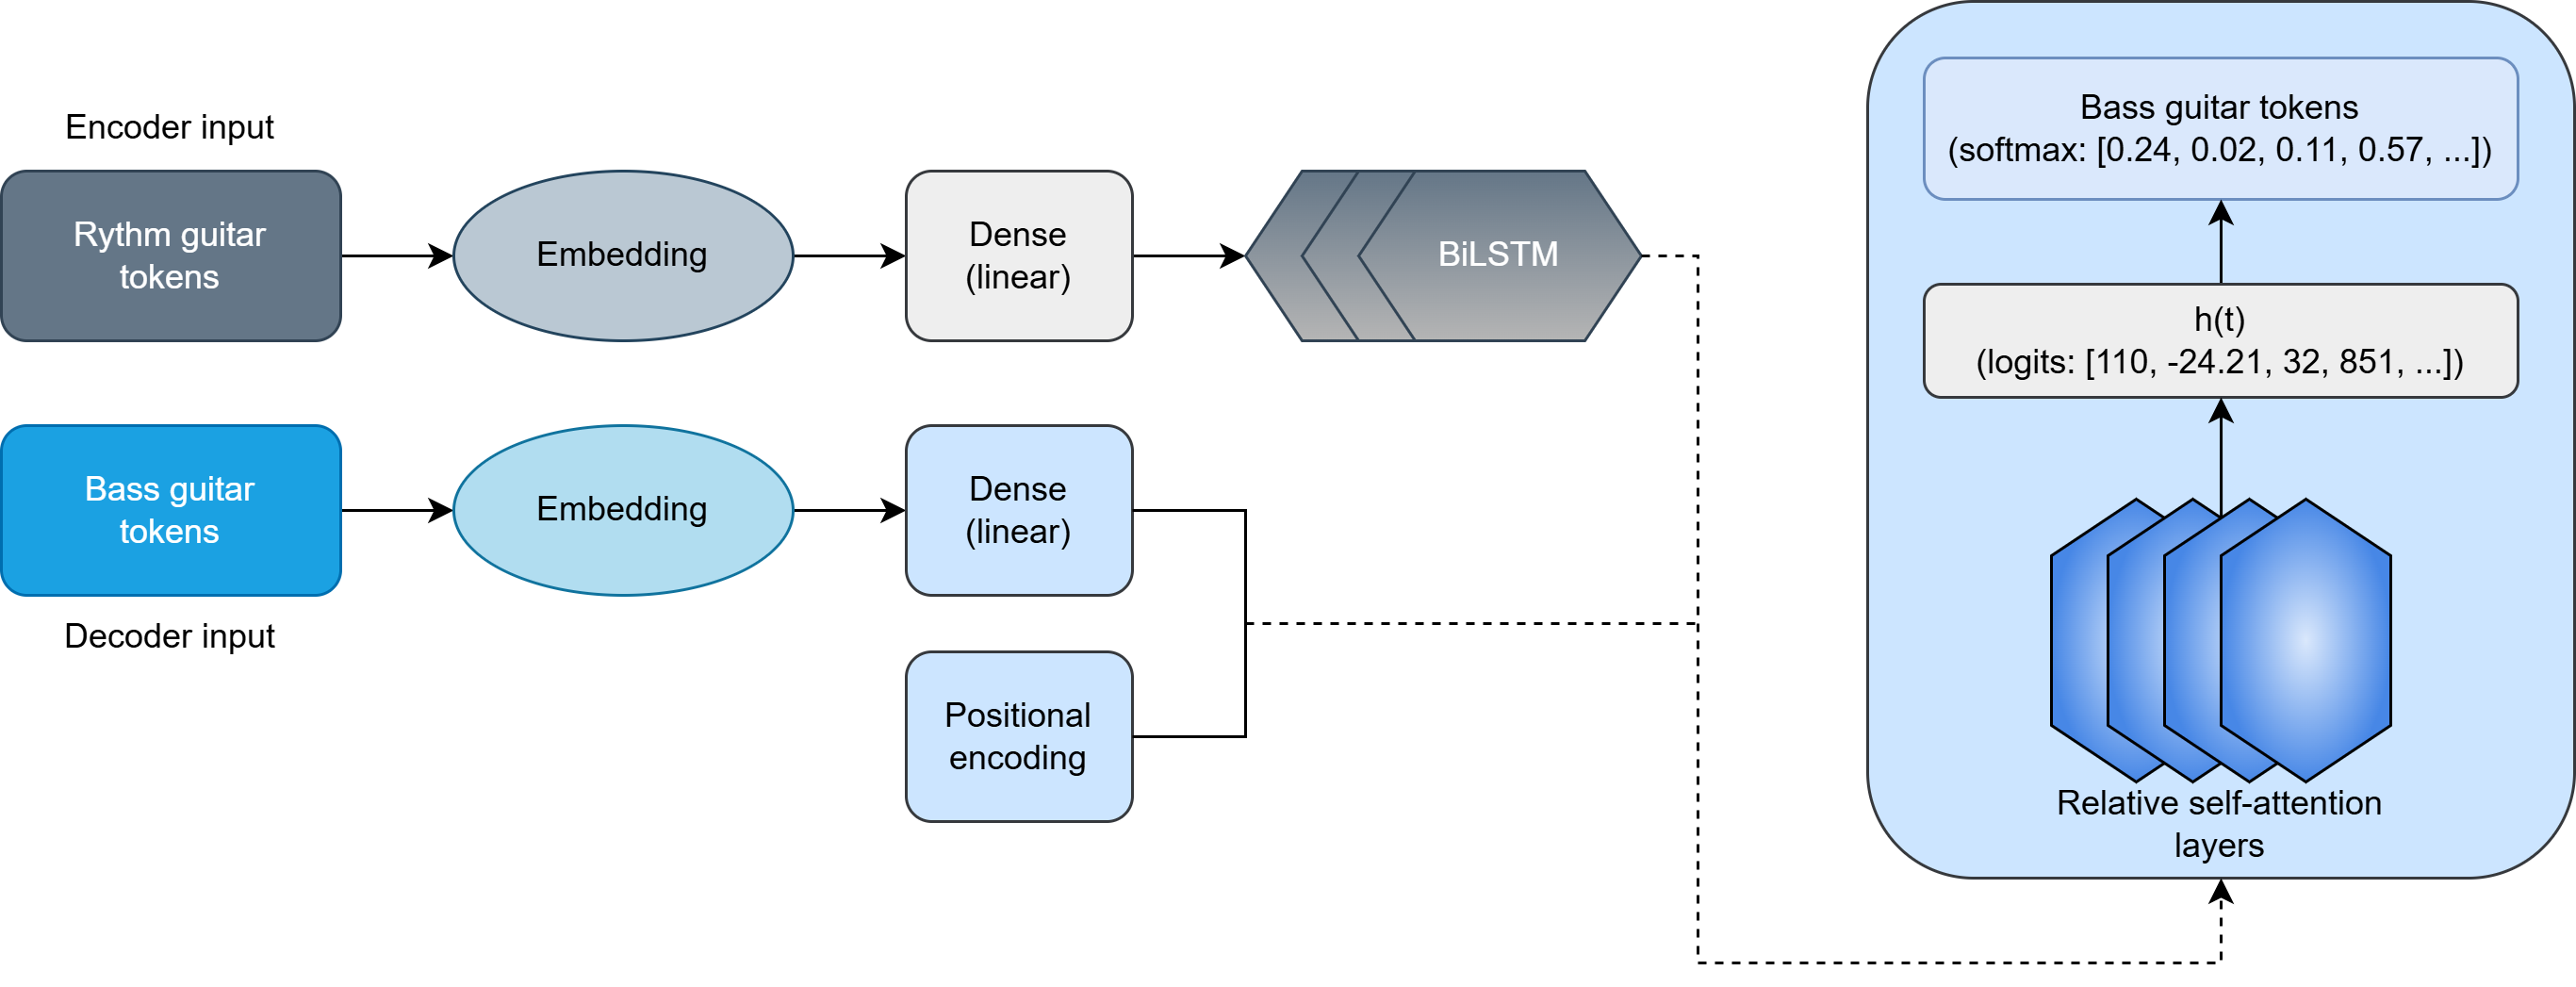
\includegraphics[width=.9\linewidth]{../images-figures/model_adapted.png}
    \caption{Makris et al. model adapted to our task}
    \label{fig:makris_model_adapted}
\end{figure}

Figure \ref{fig:makris_model_adapted} shows the model adapted to our task.
In our case, we have chosen to use DadaGP tokenization which is a different representation.
On the encoder side, the five embeddings concatenated in Makris et al. are replaced by a single embedding in our case.
On the decoder side, the compound word is only made of two inputs because drums notes need much less parameters than other instruments.
They are fully described by their onset and a value indicating the drum type.
This compound representation is also replaced by a single embedding in our case.

The Encoder processes rhythm guitar tokens using a bidirectional Long Short-Term Memory (BiLSTM) network, allowing the model to capture dependencies both forward and backward in the sequence.
The BiLSTM generates a latent variable \( z \), which encodes both rhythmic and structural information from the input sequence.
This latent variable serves as a compressed representation of the rhythm guitar part. 
The Decoder follows an autoregressive approach, predicting each token sequentially.
At each time step \( t-1 \), the Decoder receives the previously generated token, embedded through a dense layer, along with the latent variable \( z \) from the Encoder, which provides contextual information.
The Decoder is based on a Transformer architecture with self-attention layers, allowing it to model long-range dependencies within the generated sequence.
Unlike standard Transformers that rely solely on absolute positional encodings, we incorporate Relative Global Attention to enhance the model's ability to capture hierarchical musical structures.
This mechanism enables the model to account for both global position information and relative relationships between musical events, which is crucial for generating coherent bass lines that align with the rhythm guitar.  

Following prior work on relative attention, we set the relative attention window size to half of the total sequence length.
This balances local context within measures and global context across phrases, improving the overall consistency of the generated bass lines.
The final output of the Transformer Decoder consists of relation-aware self-attention activations \( h_t \), which are passed through a Dense layer followed by a softmax activation.
Our adapted model consists of approximately 21 million parameters, significantly smaller than architectures such as the Pop Music Transformer, which has around 41 million parameters~\cite{huang_pop_2020}.
This makes our approach more efficient while still capturing the necessary musical relationships.  

To evaluate our model's performance, we use a loss function based on categorical cross-entropy and an accuracy metric designed for sequence modeling.
The loss function measures how well the predicted probability distribution aligns with the true tokens and is defined as:  

\begin{equation} \label{eq:loss}
    \mathcal{L} = - \sum_{t=1}^{T} \sum_{k=1}^{K} y_{t,k} \log \hat{y}_{t,k}
\end{equation}
    
where \( T \) is the sequence length, \( K \) is the vocabulary size, \( y_{t,k} \) is the ground-truth token at time step \( t \), and \( \hat{y}_{t,k} \) is the predicted probability for token \( k \).
The ground-truth token is the token that effectively appears in the original bass guitar sequence at time step \( t \).
Our accuracy metric computes the proportion of correctly predicted tokens in a sequence.
Both functions incorporate a masking mechanism to handle padding tokens and remove their contribution to the calculations.


\subsection{Training}

Training was done on GPU with at most 200 epochs and an early-stopping criterion of 5 epochs without improvement on the validation loss.
This means that the training stops if the validation loss does not decrease for 5 consecutive epochs.
We used Adam optimizer with the following hyperparameters: $\alpha=5e^{-4}$, $\beta_1=0.9$, $\beta_2=0.98$, $epsilon=1e^{-9}$, and a batch size of 32.
The training stopped at epoch 37 because the validation loss did not decrease anymore for 5 epochs.
We reached 0.97 accuracy on the validation set with 0.14 loss.

% FIGURE EVOLUTION OF ACCURACY AND LOSS DURING TRAINING
\begin{figure}[!ht]
    \centering
    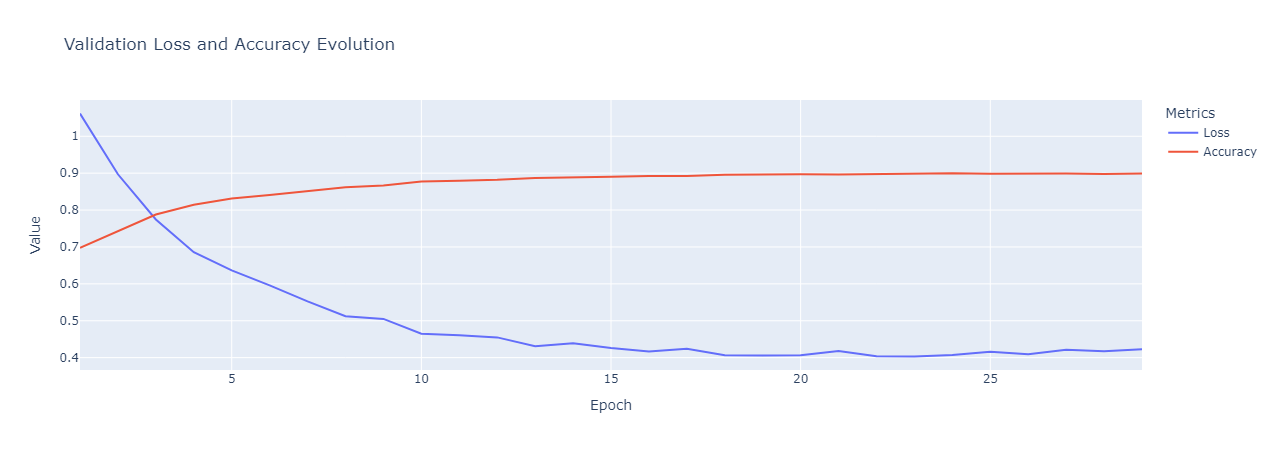
\includegraphics[width=.8\linewidth]{../images-figures/validation_acc_loss.png}
    \caption{Evolution of validation accuracy and loss during the training}
    \label{fig:validation_acc_loss}
\end{figure}

Figure \ref{fig:validation_acc_loss} shows the evolution of accuracy and loss during training.
The accuracy increases rapidly during the first epochs, then stabilizes around 0.965.